\paragraph{Página MP3}
En primer lugar, nos econtramos con una sección llamada \textit{Canciones}, la cual cuenta con un menú desplegable con lista, con sus correspondientes nombres, de las posibles canciones. Junto a dicho menú, se cuentra un botón que nos permite confimar la canción seleccionada.

A continuación, encontramos la sección demoninada \textit{Control} la cual cuentra con 4 botones. El primero, nos permite seleccionar la canción anterior a la canción acutal. A continuación, nos encontramos con un botón que nos permite tanto pausar como continuar la reproducción de la canción actual. El siguiente botón nos permite seleccionar la siguiente canción de la lista. Por último, el botón de abajo, nos permite activar y desactivar la puesta en bucle de la canción actual.

De forma análoga a la página de la Radio, las siguientes dos secciones nos permiten modificar el volumen del sistema y la salida de la señal de audio.

\begin{figure}[H]
    \centering
    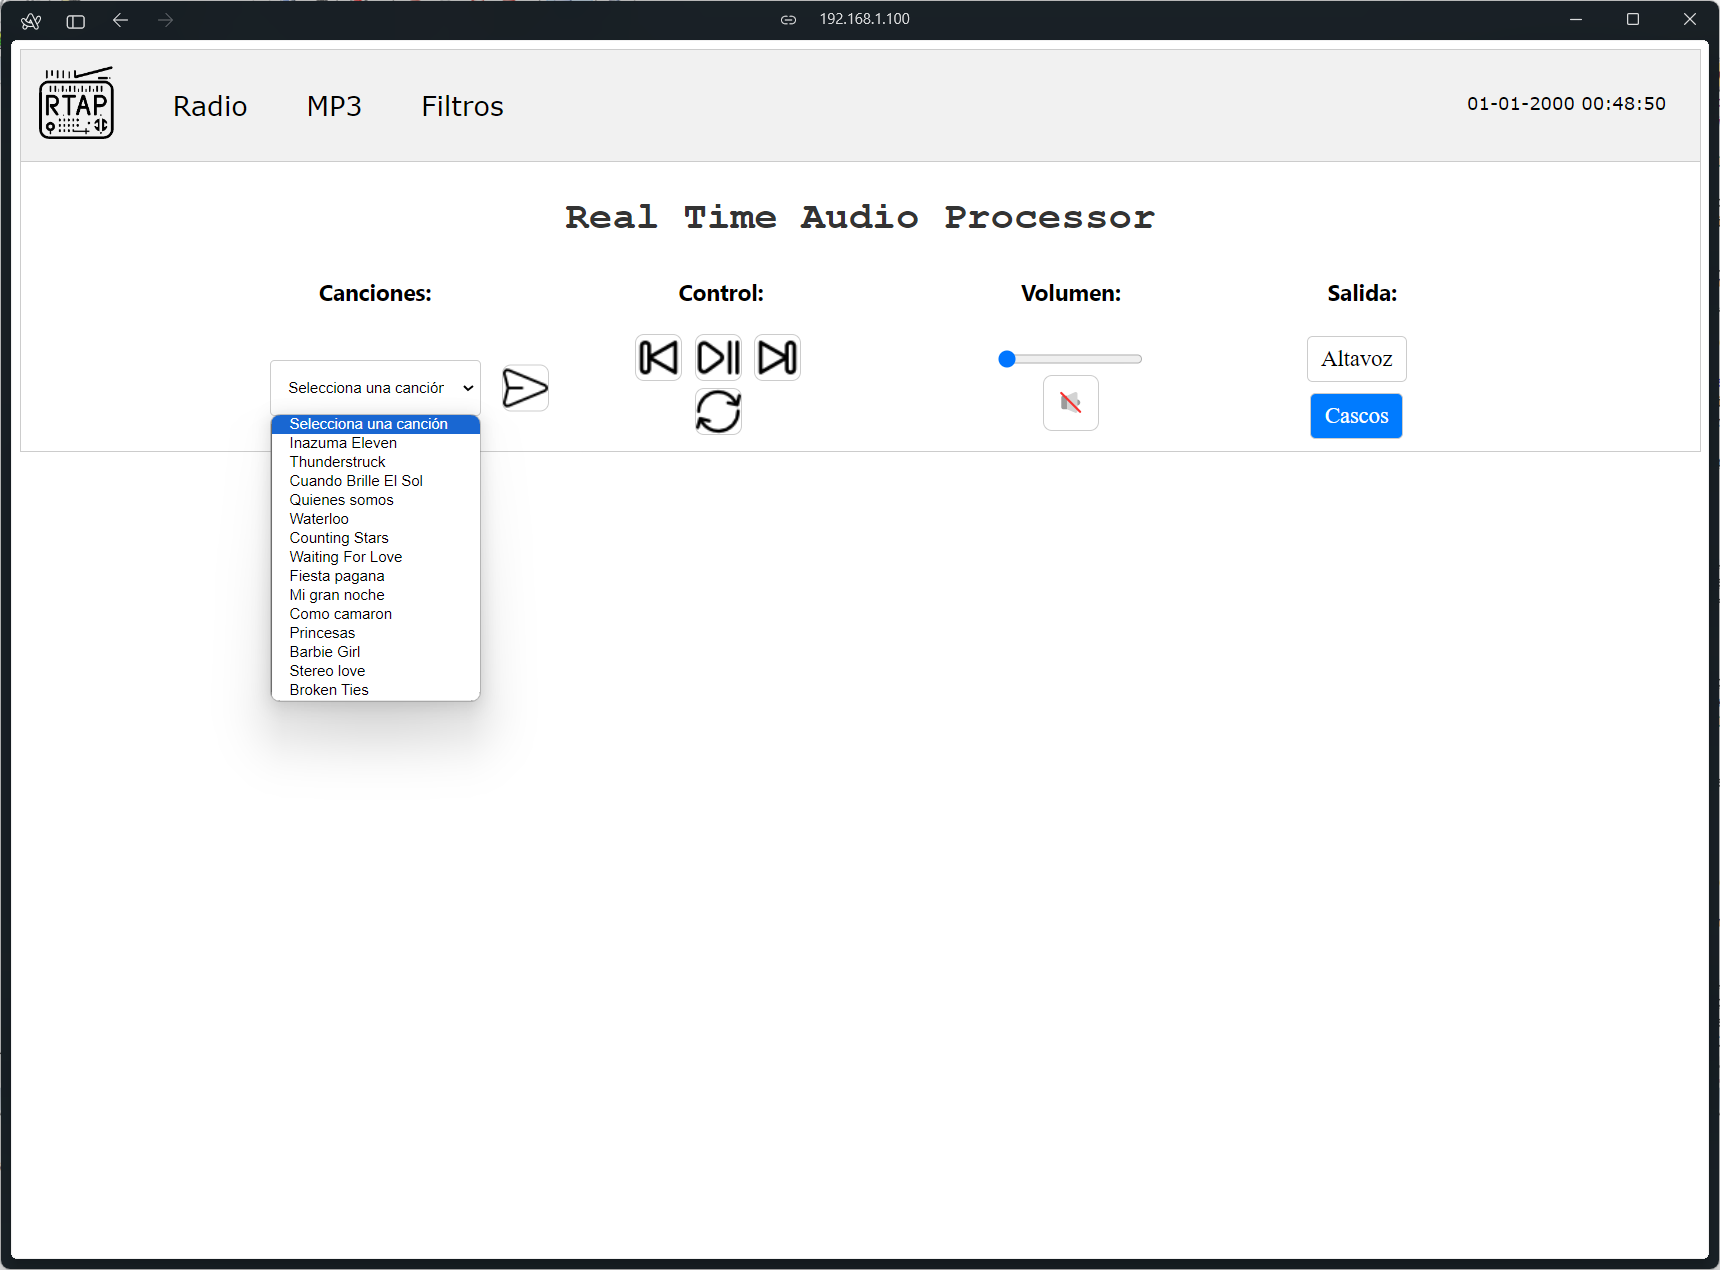
\includegraphics[width=0.8\textwidth]{images/3/3-1/3-1-1-3/Pagina_MP3.png}
    \caption{Página MP3}
    \label{fig:3-1-1-3-MP3}
\end{figure}